% ============================================================
%  EDCI 59100-016  |  Assignment 10: Draft Literature Review
%  Md Kamruzzaman Kamrul  |  Summer 2026
% ============================================================
\documentclass[10pt,letterpaper]{article}

\usepackage[margin=0.75in, top=0.85in, bottom=0.85in]{geometry}
\usepackage{array}
\usepackage{booktabs}
\usepackage{longtable}
\usepackage{tabularx}
\usepackage{pdflscape}
\usepackage[table]{xcolor}
\usepackage{titlesec}
\usepackage{fancyhdr}
\usepackage{enumitem}
\usepackage{microtype}
\usepackage[hidelinks]{hyperref}
\usepackage{tikz}
\usepackage{pgfplots}
\pgfplotsset{compat=1.17}
\usepackage{pgf-pie}
\usetikzlibrary{shapes.geometric, arrows.meta, positioning, fit, calc}
\usepackage{setspace}
\usepackage{caption}
\usepackage{subcaption}
\usepackage{float}
\usepackage{amsmath}
\usepackage{graphicx}
\usepackage{multirow}

\definecolor{headingblue}{HTML}{1F4E79}
\definecolor{lightblue}{HTML}{D9EAF7}
\definecolor{softgray}{HTML}{F4F6F8}
\definecolor{darkgray}{HTML}{404040}
\definecolor{prismagreen}{HTML}{E8F5E9}
\definecolor{prismabox}{HTML}{1565C0}
\definecolor{chartblue}{HTML}{2196F3}
\definecolor{chartorange}{HTML}{FF9800}
\definecolor{chartgreen}{HTML}{4CAF50}
\definecolor{chartred}{HTML}{F44336}
\definecolor{chartpurple}{HTML}{9C27B0}
\definecolor{chartgray}{HTML}{9E9E9E}

\pagestyle{fancy}
\fancyhf{}
\lhead{\small Md Kamruzzaman Kamrul}
\chead{\small EDCI 59100-016 \textbar{} Draft Literature Review}
\rhead{\small Summer 2026}
\cfoot{\small \thepage}
\renewcommand{\headrulewidth}{0.4pt}
\setlength{\headheight}{14pt}

\titleformat{\section}{\normalfont\large\bfseries\color{headingblue}}{\thesection.}{0.5em}{}
\titleformat{\subsection}{\normalfont\normalsize\bfseries\color{headingblue}}{\thesubsection.}{0.5em}{}
\titleformat{\subsubsection}{\normalfont\normalsize\bfseries\color{darkgray}}{\thesubsubsection.}{0.45em}{}
\titlespacing*{\section}{0pt}{11pt}{4pt}
\titlespacing*{\subsection}{0pt}{8pt}{3pt}
\titlespacing*{\subsubsection}{0pt}{6pt}{2pt}

\setlength{\parindent}{0pt}
\setlength{\parskip}{5pt}
\setlist[itemize]{leftmargin=*,itemsep=2pt,topsep=2pt}
\setlist[enumerate]{leftmargin=*,itemsep=2pt,topsep=2pt}
\renewcommand{\arraystretch}{1.18}
\setlength{\tabcolsep}{4pt}
\emergencystretch=3em

\newcolumntype{L}[1]{>{\raggedright\arraybackslash}p{#1}}
\newcolumntype{Y}{>{\raggedright\arraybackslash}X}

\captionsetup{font=small, labelfont=bf}

% ============================================================
\begin{document}

\begin{center}
{\Large\bfseries\color{headingblue} Vision-Language Models for Construction Site Safety and Progress Monitoring: A Scoping Review}\\[0.4em]
{\normalsize Draft Literature Review Paper --- Week 5 Submission}\\[0.2em]
{\normalsize Md Kamruzzaman Kamrul}\\
{\normalsize EDCI 59100-016 \textbar{} Summer 2026}\\[0.2em]
{\small \textit{Submitted for peer review and instructor feedback. Assignment 10.}}\\[0.25em]
{\small Discipline: Civil Engineering / Construction Management \textbar{} Academic format: Numbered citation style consistent with \textit{Automation in Construction} (Elsevier)}
\end{center}

\vspace{0.5em}

% ============================================================
\section{Introduction}
% ============================================================

Construction sites are dynamic environments where workers, equipment, and machines operate simultaneously under conditions that make monitoring both necessary and difficult \cite{alaloul2022}. Unlike aerospace or automotive manufacturing, construction is labor-intensive, project-specific, and organized around ad-hoc supply chains. These characteristics render standard industrial monitoring systems impractical \cite{davila2021,alaloul2022}.

Site managers carry two parallel responsibilities: keeping the environment hazard-free through regular safety inspection \cite{asadzadeh2020}, and tracking activity progress against production targets \cite{alaloul2022}. Both tasks rely on manual observation---physical walk-throughs, visual hazard checks, hand-logged Daily Construction Reports (DCRs), which are subjective, error-prone, and slow \cite{samsami2024,alaloul2022}.

The resulting information lag impairs schedule and cost monitoring and limits managers' ability to detect variability before it compounds \cite{alaloul2022}. These bottlenecks explain the industry's persistent safety and productivity challenges \cite{jiang2023}, and have driven growing adoption of AI---particularly computer vision---as an automated alternative \cite{rabbi2024,paneru2021}.

To overcome the data deficiencies of traditional manual methods, research initially shifted toward automated object-level data collection \cite{tuomisto2026}. Rather than broadly applying automation to all construction tasks, this specific technological domain focused on developing automated, real-time performance monitoring systems consisting of location tracking, activity recognition, and performance monitoring \cite{sherafat2020}. To achieve this, the first of these methods involved attaching tracking devices like Radio Frequency Identification (RFID), Ultra-Wideband (UWB), or Bluetooth Low Energy (BLE) to building components \cite{asadzadeh2020}. However, while these tag-based methods are effective for locating materials, they cannot verify the proper installation or condition of components, limiting their utility for detailed inspection tasks \cite{sherafat2020}. Furthermore, tracking eventually thousands of items does not offer an economical or practical approach in large-scale projects \cite{bohn2010}. The field therefore adopted computer vision techniques. Cameras require no sensor attachments and capture the locations and activities of construction entities, providing both operational and technical advantages over wearable-sensor systems \cite{xiong2019}.

Building upon the shift toward camera-based monitoring, the field widely deployed traditional computer vision approaches utilizing bounding-box detectors to locate construction entities. While these models are highly effective at spatial localization, identifying only the workers and PPE components, without recognizing the contextual relationship between them, does not effectively verify PPE compliance \cite{nath2020}. Specifically, inferring that workers are prone to experience falling from height based on safety regulations is difficult for computer vision; this condition can be summarized as a \textit{semantic gap}---a term applied to the construction compliance context by Wu et al.\ \cite{wu2021}. Because computer vision cannot natively comprehend safety rulebooks, traditional pipelines attempted to bridge this gap by applying an algorithm with explicit rules determined through empirical observations \cite{nath2020}. However, manually establishing these rules for multiple PPEs is a complicated task and results may not be structured or comprehensive enough to consider all possible scenarios \cite{nath2020}.

To overcome the limitation of manual geometric mapping, research explored an alternative approach using Natural Language Processing (NLP) for automatically extracting regulatory requirements from textual regulatory documents and formalizing these requirements in a logic format \cite{zhang2015}. Yet, while NLP excels at rule extraction, these text-based models are fundamentally blind to the physical site. Ultimately, they simply represent the extracted safety requirements in the form of query graphs for supporting subsequent knowledge graph-based field compliance checking \cite{wang2023}. Consequently, this creates a profound technological disconnect: computer vision can see the site but cannot understand the rules, while NLP understands the rules but cannot see the site. This fundamental limitation necessitates the emergence of multimodal Vision-Language Models (VLMs) capable of natively fusing both data streams.

To address the fundamental limitations of traditional methods in processing semantic information, recent advancements have introduced multi-modal large language models (MLLMs), upon which vision-language models (VLMs) combine image processing and natural language processing (NLP) \cite{chan2025}. By extracting both intricate visual and linguistic features, these models can perform multiple types of instruction-following tasks such as image captioning, visual grounding, and visual question answering (VQA) \cite{chan2025}. Furthermore, these architectures acquire generalized visual representations guided by natural language supervision, enabling impressive zero-shot detection capabilities \cite{zhang2025}. By leveraging natural language prompts and contextual reasoning, VLMs offer a flexible approach for spatiotemporal analysis. They interpret both the spatial geometry of hazards and the temporal sequence of complex human behaviors on dynamic construction sites, potentially reducing dependence on extensive labeled datasets \cite{bui2026}. Consequently, these multimodal systems can create human-readable captions for daily progress and work activity logs \cite{jung2024}, while simultaneously supporting interactive question-and-answer sessions, fostering a more informed understanding of construction site safety \cite{hussain2026}.

Despite the rapid emergence of VLMs as a paradigm-shifting technology, existing reviews have remained siloed in their respective unimodal domains. The majority of existing reviews on AI applications in the construction industry tend to focus on specific domains within AI, such as computer vision or NLP, thereby addressing only fragments of the potential AI applications \cite{rabbi2024}. For instance, previous reviews have extensively mapped pure computer vision research in construction \cite{jiang2023,paneru2021,zhong2019} or provided overviews of sensor-based safety management \cite{asadzadeh2020}. While these studies provide valuable baselines, existing reviews do not cover the latest technological advances and lack systematic elaboration for construction scene understanding \cite{zhang2025}. Specifically, although Vision-Language Models (VLMs) excel in general multimodal tasks, their ability to understand human behavior in safety-critical construction environments remains largely unexplored \cite{bui2026}. Due to the development of scene understanding and large language models in recent years, it is necessary to conduct a new review on this topic to capture these paradigm-shifting advancements \cite{zhang2025}.

To address this critical gap, this paper presents a comprehensive scoping review of multimodal vision-language systems applied to construction safety and progress monitoring. Conducted in strict accordance with the PRISMA-ScR guidelines \cite{tricco2018}, the specific objectives of this study are to: (1) map the current landscape of VLM applications in construction management; (2) develop a robust taxonomy bridging foundational VLM architectures with practical construction management applications; and (3) analyze existing algorithmic limitations to outline a roadmap for future research in construction. To achieve these objectives, this review seeks to explicitly answer the following four primary research questions (RQs):

\begin{itemize}
  \item \textbf{RQ1:} What are the prevalent Vision-Language Model (VLM) architectures currently utilized for spatiotemporal analysis in construction?
  \item \textbf{RQ2:} How is multimodal data (visual and textual) fused and processed across construction safety and progress monitoring applications?
  \item \textbf{RQ3:} What are the primary methodological bottlenecks in deploying these models for real-time progress tracking and safety?
  \item \textbf{RQ4:} How is the performance of Vision-Language Models currently evaluated and benchmarked for spatiotemporal tasks in construction?
\end{itemize}

% ============================================================
\section{Research Methodology}
% ============================================================

This review was conducted in accordance with the PRISMA-ScR (Preferred Reporting Items for Systematic Reviews and Meta-Analyses extension for Scoping Reviews) guidelines \cite{tricco2018}. This review adopts a scoping design rather than quantitative meta-analysis for two reasons. First, VLMs represent an emerging architecture whose extent, range, and nature in construction applications requires mapping before any narrow intervention comparison is appropriate \cite{chan2025,chen2024}. Second, the included studies use heterogeneous evaluation metrics: geometric precision measures such as mean Average Precision \cite{nath2020,wang2024} alongside natural language generation metrics such as BLEU and CIDEr \cite{jung2024,xiao2022}. This heterogeneity makes standardized statistical synthesis impossible.

\subsection{Search Strategy and Information Sources}

To ensure a rigorous and reproducible retrieval process, the literature search was conducted on 4\textsuperscript{th} March 2026 across two of the most comprehensive scientific databases for engineering and computer science research: the Web of Science (WoS) Core Collection and Scopus. These specific databases were selected because WoS contains the most comprehensive and influential journals within the field of construction and engineering management \cite{zhong2019}, and Scopus is actively used alongside WoS as a primary search engine for AI applications in the construction domain \cite{rabbi2024}. The keywords were determined by analyzing frequent words found in papers where AI was applied to enhance construction management and safety \cite{rabbi2024}. The search query was constructed using a tripartite Boolean logic framework designed to intersect three distinct conceptual domains: (1) the specific AI architecture, (2) the analytical task, and (3) the application domain. The exact search strings applied across both databases are as follows:

\begin{quote}
\textbf{String 1 --- AI Architecture:} (``Vision-Language Model*'' OR ``VLM'' OR ``Vision-Text'' OR ``Image-Text'' OR ``Visual Question Answering'' OR ``VQA'' OR ``Image Captioning'' OR ``CLIP'' OR ``Large Multimodal Model*'' OR ``LMM'' OR ``Foundation Model*'' OR ``Generative AI'' OR ``Video-Language'' OR ``Video-Text'') AND

\textbf{String 2 --- Analytical Task:} (``Spatiotemporal'' OR ``Spatio-temporal'' OR ``Video'' OR ``Temporal'' OR ``Dynamic'' OR ``Time-series'' OR ``4D'' OR ``Motion'' OR ``Tracking'' OR ``Sequenc*'' OR ``Action recognition'' OR ``Activity recognition'') AND

\textbf{String 3 --- Application Domain:} (``Construction Management'' OR ``Civil Engineering'' OR ``AEC'' OR ``Infrastructure'' OR ``Built Environment'' OR ``Construction Site'' OR ``Safety Monitoring'' OR ``Structural Health Monitoring'' OR ``Digital Twin'')
\end{quote}

Given the rapidly evolving nomenclature of VLM research, relying purely on an algorithmic, keyword-based search poses a risk of omitting foundational or transitional works that may not employ contemporary terminology. To address this limitation, a secondary backward snowballing (ancestry/reference chain) strategy was employed. The reference lists of all articles retained after the full-text review were systematically mined to identify foundational or transitional technologies, ensuring that articles missed during the keyword search process were identified from reference chains \cite{rabbi2024}.

\subsection{Eligibility Criteria}

To maintain a disciplined and reproducible scope in accordance with the PRISMA-ScR guidelines \cite{tricco2018}, explicit inclusion and exclusion criteria were established a priori, prior to the commencement of the screening process. These criteria were strategically designed to isolate high-quality literature that directly addresses the intersection of multimodal AI and active construction management. Furthermore, the criteria deliberately retain a select number of traditional unimodal Computer Vision (CV) and Natural Language Processing (NLP) papers to establish an evolutionary comparative baseline. This baseline is essential to empirically demonstrate the inherent limitations of prior technologies and the ``semantic gap'' \cite{wu2021}. The criteria applied during the screening process are summarized in Table~\ref{tab:inclusion}.

\begin{table}[H]
\caption{Summary of Inclusion and Exclusion Criteria.}
\label{tab:inclusion}
\small
\rowcolors{2}{softgray}{white}
\begin{tabularx}{\textwidth}{L{2.6cm} Y Y}
\toprule
\rowcolor{lightblue}
\textbf{Dimension} & \textbf{Inclusion Criteria} & \textbf{Exclusion Criteria}\\
\midrule
Publication Date & 2019--2026 (core VLM literature); 2010--2026 (foundational CV baselines). & Pre-2010; post-March 2026. \\
Source Type & High-impact peer-reviewed journal. & Editorials, book chapters, theses, non-English documents, conference proceedings, and industry white papers. \\
Technology & Multimodal architecture integrating visual/geometric data with textual/semantic data (VLMs, VQA, image captioning, CLIP-based models, MLLMs). & Purely unimodal CV or purely text-based NLP, unless serving as an explicit comparative baseline within a hybrid framework. \\
Application Domain & Active construction phase: safety management (hazard identification, PPE compliance) and progress tracking (productivity analysis, schedule monitoring, reporting). & Post-construction, facility management, structural health monitoring, or non-engineering domains. \\
\bottomrule
\end{tabularx}
\end{table}

\textit{Note on source eligibility:} One paper in the corpus---Bui et al.\ (2026)---is available as an arXiv preprint and has not undergone formal peer review at the time of this search. It is retained for its direct relevance to the review's core question (evaluating VLM performance on construction worker recognition) but should be interpreted with awareness of its pre-review status.

\subsection{Selection of Sources of Evidence}

The selection process for sources of evidence was conducted in two sequential phases---primary database retrieval and backward snowballing---and is visually summarized in the PRISMA-ScR flow diagram (Figure~\ref{fig:prisma}).

During Phase 1, the initial query across Web of Science and Scopus yielded 1,443 raw records (769 from WoS and 674 from Scopus). Automated database filters restricting results to relevant subject areas, the English language, and peer-reviewed document types excluded 1,320 records, leaving 123 articles. After removing 33 duplicate records, 90 unique articles remained for manual screening. A rigorous two-stage manual screening protocol was subsequently employed. In the first stage, title and abstract screening resulted in the exclusion of 32 articles that fell outside the scope of the active construction context. The remaining 58 articles were advanced to full-text review. During this second stage, 33 articles were excluded due to an exclusive focus on domains outside the active construction phase, insufficient methodological detail regarding multimodal architectures, or reliance on unimodal architectures that did not belong to the baseline-to-VLM progression. This rigorous filtration process yielded a Phase 1 dataset of 25 core VLM and transitional articles.

Concurrently, Phase 2 was executed via backward snowballing of the retained articles, successfully identifying an additional 31 highly relevant baseline and transition articles. Integrating both phases culminated in a final corpus of \textbf{56 articles}, comprising 31 baseline/background papers, 5 transition/bridging papers, and 20 core construction VLM papers.

\begin{figure}[H]
\caption{PRISMA-ScR Flow Diagram for Study Selection.}
\label{fig:prisma}
\centering
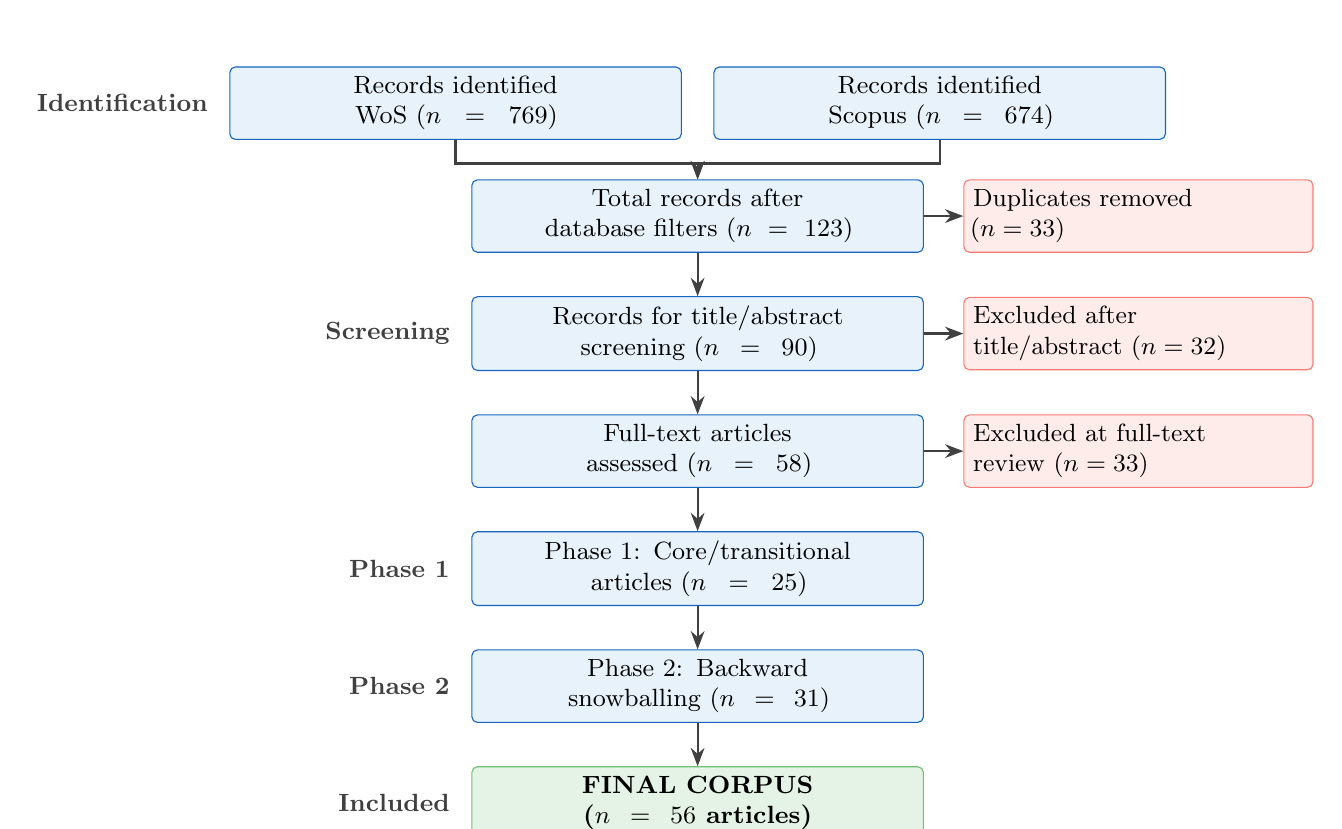
\begin{tikzpicture}[
  box/.style={rectangle, draw=prismabox, fill=lightblue!60, text width=5.5cm, align=center, minimum height=0.75cm, font=\small, rounded corners=2pt},
  excl/.style={rectangle, draw=chartred!70, fill=chartred!10, text width=4.2cm, align=left, minimum height=0.7cm, font=\small, rounded corners=2pt},
  final/.style={rectangle, draw=chartgreen!80, fill=chartgreen!15, text width=5.5cm, align=center, minimum height=0.8cm, font=\small\bfseries, rounded corners=2pt},
  arr/.style={-Stealth, thick, color=darkgray},
  node distance=0.65cm
]

% Identification
\node[box] (wos) {Records identified\\ WoS ($n=769$)};
\node[box, right=0.4cm of wos] (scop) {Records identified\\ Scopus ($n=674$)};
\node[box, below=0.5cm of $(wos.south)!0.5!(scop.south)$] (total) {Total records after\\ database filters ($n=123$)};
\node[excl, right=0.5cm of total] (dup) {Duplicates removed\\ ($n=33$)};

\draw[arr] (wos.south) -- ++(0,-0.3) -| (total.north);
\draw[arr] (scop.south) -- ++(0,-0.3) -| (total.north);
\draw[arr] (total.east) -- (dup.west);

% Screening
\node[box, below=0.55cm of total] (screen) {Records for title/abstract\\ screening ($n=90$)};
\node[excl, right=0.5cm of screen] (excl1) {Excluded after\\ title/abstract ($n=32$)};

\draw[arr] (total.south) -- (screen.north);
\draw[arr] (screen.east) -- (excl1.west);

\node[box, below=0.55cm of screen] (fulltext) {Full-text articles\\ assessed ($n=58$)};
\node[excl, right=0.5cm of fulltext] (excl2) {Excluded at full-text\\ review ($n=33$)};

\draw[arr] (screen.south) -- (fulltext.north);
\draw[arr] (fulltext.east) -- (excl2.west);

% Phase 1 result
\node[box, below=0.55cm of fulltext] (phase1) {Phase 1: Core/transitional\\ articles ($n=25$)};
\draw[arr] (fulltext.south) -- (phase1.north);

% Phase 2 snowball
\node[box, below=0.55cm of phase1] (snowball) {Phase 2: Backward\\ snowballing ($n=31$)};
\draw[arr] (phase1.south) -- (snowball.north);

% Final
\node[final, below=0.55cm of snowball] (final) {FINAL CORPUS\\ ($n=56$ articles)};
\draw[arr] (snowball.south) -- (final.north);

% Labels
\node[font=\small\bfseries\color{darkgray}, left=0.15cm of wos.west, align=right] {Identification};
\node[font=\small\bfseries\color{darkgray}, left=0.15cm of screen.west, align=right] {Screening};
\node[font=\small\bfseries\color{darkgray}, left=0.15cm of phase1.west, align=right] {Phase 1};
\node[font=\small\bfseries\color{darkgray}, left=0.15cm of snowball.west, align=right] {Phase 2};
\node[font=\small\bfseries\color{darkgray}, left=0.15cm of final.west, align=right] {Included};

\end{tikzpicture}
\end{figure}

\subsection{Data Charting and Extraction Process}

Following the selection of the 56 core articles, a standardized data extraction framework was developed to systematically chart the literature. As recommended by scoping review methodologies \cite{tricco2018}, the data charting form was iteratively refined to ensure all relevant variables addressing the research questions were captured consistently. To provide a structured and comprehensive evaluation, the extracted data were systematically categorized into three distinct analytical dimensions: Content Analysis, Technical Analysis, and Critical Analysis. The complete data charting framework is detailed in Table~\ref{tab:charting}. Data charting was conducted by the primary researcher; no independent dual-review or inter-rater reliability calculation was performed, which represents a methodological limitation acknowledged in Section~\ref{sec:discussion}.

\begin{table}[H]
\caption{Data Charting and Extraction Framework.}
\label{tab:charting}
\small
\rowcolors{2}{softgray}{white}
\begin{tabularx}{\textwidth}{L{2.6cm} L{4.5cm} Y}
\toprule
\rowcolor{lightblue}
\textbf{Analytical Dimension} & \textbf{Extraction Variables} & \textbf{Description}\\
\midrule
Content Analysis & Cluster/Application; Input Data; Spatiotemporal Task; Automation Level. & Identifies what the AI is doing by mapping the specific domain (e.g., safety vs.\ progress tracking), the sensory inputs utilized (e.g., video, image, point cloud), the specific spatiotemporal task (e.g., action recognition, tracking), and the system's level of autonomy (assistive vs.\ automated).\\
Technical Analysis & Algorithm/Model; Dataset; Validation Metric; Compute/Hardware. & Analyzes how the system operates by documenting the specific architectures (e.g., GPT-4o, CLIP), the nature of the training data (public vs.\ private/custom), the diverse evaluation metrics employed (e.g., mAP, F1-score), and the deployment environment (edge vs.\ cloud).\\
Critical Analysis & Key Limitation; Research Gap; Future Direction. & Evaluates the significance of the study by synthesizing the inherent technological or methodological bottlenecks, identifying unmet industry needs, and charting actionable future research trajectories.\\
\bottomrule
\end{tabularx}
\end{table}

\subsection{Data Synthesis}

Given the heterogeneous nature of the evaluation metrics across included studies---which range from geometric intersection-over-union (IoU) and mean average precision (mAP) metrics \cite{nath2020,wang2024} to semantic fluency metrics for evaluating image captioning models, such as BLEU, METEOR, and CIDEr \cite{jung2024,xiao2022}---a standardized quantitative meta-analysis was deemed inappropriate. Instead, a thematic and narrative synthesis approach was adopted \cite{tricco2018}. The final corpus of 56 papers was thematically classified into three distinct developmental stages: (1) the traditional baseline establishing the geometric-semantic disconnect, (2) the transitional bridge leveraging advanced but unimodal algorithms, and (3) the paradigm shift toward end-to-end Vision-Language Models (VLMs). This thematic categorization forms the structural foundation for the subsequent descriptive and thematic analyses presented in Sections~3 and~4.

% ============================================================
\section{Descriptive Analysis of the Corpus}
% ============================================================

This chapter presents the descriptive mapping of the 56-article corpus and directly addresses the PRISMA-ScR requirement to characterize the volume, nature, and distribution of the included evidence. The analysis maps the body of literature across temporal, geographic, journal, methodological, and topical dimensions---establishing the empirical foundation upon which the thematic analysis in Section~4 is built.

\subsection{Corpus Composition and Overview}

The final 56-paper corpus is methodologically stratified into three developmental tiers: 31 baseline and background studies (55.4\%), 5 transitional bridge studies (8.9\%), and 20 core construction VLM studies (35.7\%). The baseline tier encompasses sensor-based tracking, unimodal computer vision, and NLP-based compliance systems that establish the technological trajectory leading to VLMs. The transition tier captures studies deploying transformer-based architectures or hybrid CV--NLP pipelines that bridged the semantic gap prior to the full multimodal turn. The core VLM tier represents recent studies deploying CLIP, MLLM, captioning, and agentic hybrid stacks for active construction scene understanding.

\textbf{Analytical scope clarification:} The 56-paper corpus is reported in full in this descriptive chapter to satisfy PRISMA-ScR's requirement that all included evidence be characterized. However, the primary analytical sample for the thematic analysis in Section~4 comprises only the \textbf{25 Phase~1 papers} (20 core VLM studies + 5 transition/bridging studies) retrieved through the direct database search. The remaining 31 Phase~2 baseline papers---identified via backward snowballing---are included solely to establish the pre-VLM technological baseline and are used only for contextual reference and discussion, not as primary evidence.

\subsection{Publication Trends and Temporal Evolution}

Figure~\ref{fig:pubyear} illustrates the temporal distribution of the 56 included papers across the review window. Publications prior to 2019 (two papers from 2010 and 2015) serve exclusively as methodological baseline anchors. A modest but steady accumulation is observed from 2019 through 2022, with the field recording fewer than eight papers per year during this period---reflecting the dominance of unimodal CV approaches and early transformer experiments. The pattern shifts decisively from 2023 onward, with 8 papers in 2023, 11 in 2024, 11 in 2025, and 5 already identified by the March 2026 search cutoff. This acceleration closely corresponds to the public release of large-scale multimodal foundation models (e.g., GPT-4V, CLIP, Florence-2, LLaVA) beginning in 2022--2023, which rapidly lowered the barrier to deploying VLMs on domain-specific applications.

\begin{figure}[H]
\caption{Annual distribution of included publications (2010--2026). Rapid growth after 2022 reflects the proliferation of foundational VLM architectures.}
\label{fig:pubyear}
\centering
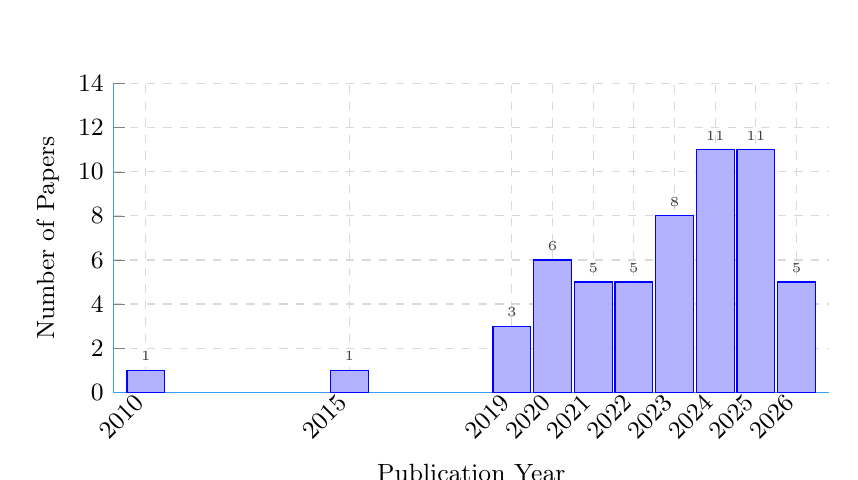
\begin{tikzpicture}
\begin{axis}[
  ybar,
  bar width=0.48cm,
  width=0.88\textwidth,
  height=5.5cm,
  xlabel={Publication Year},
  ylabel={Number of Papers},
  xtick={2010,2015,2019,2020,2021,2022,2023,2024,2025,2026},
  xticklabels={2010,2015,2019,2020,2021,2022,2023,2024,2025,2026},
  xticklabel style={rotate=45, anchor=east, font=\small},
  yticklabel style={font=\small},
  xlabel style={font=\small},
  ylabel style={font=\small},
  ymin=0, ymax=14,
  ytick={0,2,4,6,8,10,12,14},
  nodes near coords,
  nodes near coords style={font=\tiny, color=darkgray},
  axis lines*=left,
  enlarge x limits=0.05,
  fill=chartblue!70,
  draw=chartblue!90,
  tick align=inside,
  grid=major,
  grid style={dashed, gray!30},
]
\addplot coordinates {
  (2010,1) (2015,1) (2019,3) (2020,6) (2021,5) (2022,5) (2023,8) (2024,11) (2025,11) (2026,5)
};
\end{axis}
\end{tikzpicture}
\end{figure}

\subsection{Geographic Distribution}

Table~\ref{tab:geography} presents the geographic distribution of included studies based on the primary institutional affiliation of the corresponding author. East Asian institutions dominate the corpus, with China contributing the largest single-country share (20 papers, 35.7\%), followed by the United States (13 papers, 23.2\%) and South Korea (6 papers, 10.7\%). Hong Kong, Australia, Taiwan, and European institutions contribute smaller but meaningful portions. This geographic concentration reflects the broader pattern in construction AI research, where East Asian institutions---particularly those in mainland China and Hong Kong---have driven large-scale empirical studies on computer vision-based site monitoring, while U.S.-based researchers have contributed extensively to foundational methodology, activity recognition, and review studies.

\begin{table}[H]
\caption{Geographic Distribution of Included Studies by Corresponding Author Institution.}
\label{tab:geography}
\small
\rowcolors{2}{softgray}{white}
\begin{tabularx}{\textwidth}{L{3.5cm} L{1.8cm} L{2.2cm} Y}
\toprule
\rowcolor{lightblue}
\textbf{Region / Country} & \textbf{Papers ($n$)} & \textbf{Percentage} & \textbf{Representative Studies}\\
\midrule
China (Mainland) & 20 & 35.7\% & Zhong et al.\ 2019; Wu et al.\ 2021; Li et al.\ 2025\\
United States & 13 & 23.2\% & Nath et al.\ 2020; Sherafat et al.\ 2020; Paneru \& Jeelani 2021\\
South Korea & 6 & 10.7\% & Hussain et al.\ 2026; Jeoung et al.\ 2025; Jang et al.\ 2025\\
Hong Kong & 5 & 8.9\% & Chan et al.\ 2025; Liang et al.\ 2024\\
Australia & 4 & 7.1\% & Asadzadeh et al.\ 2020; Davila Delgado \& Oyedele 2021\\
Taiwan & 3 & 5.4\% & Xiao et al.\ 2022; Xiao et al.\ 2024\\
Europe (Finland, other) & 3 & 5.4\% & Tuomisto et al.\ 2026\\
Other & 2 & 3.6\% & Mixed affiliations\\
\bottomrule
\multicolumn{4}{l}{\small \textit{Total:} $n = 56$. Classification by primary corresponding author institution.}
\end{tabularx}
\end{table}

\subsection{Journal Landscape}

The 56 included studies were published across 14 distinct peer-reviewed journals. Table~\ref{tab:journals} summarizes the journal distribution. \textit{Automation in Construction} (Elsevier) is the dominant outlet, hosting 28 of the 56 papers (50.0\%), confirming its role as the primary venue for empirical construction AI research. \textit{Journal of Construction Engineering and Management} (ASCE) and \textit{Computer-Aided Civil and Infrastructure Engineering} (Wiley) contribute the next largest shares. This concentration in a small number of high-impact journals---particularly \textit{Automation in Construction}---indicates tight thematic coherence in the literature and validates the relevance of the chosen search strategy.

\begin{table}[H]
\caption{Distribution of Included Studies Across Publication Venues.}
\label{tab:journals}
\small
\rowcolors{2}{softgray}{white}
\begin{tabularx}{\textwidth}{Y L{1.8cm} L{2.2cm} L{3.8cm}}
\toprule
\rowcolor{lightblue}
\textbf{Journal} & \textbf{Publisher} & \textbf{Papers ($n$)} & \textbf{Scope Relevance}\\
\midrule
Automation in Construction & Elsevier & 28 (50.0\%) & Primary construction AI venue\\
Journal of Construction Engineering and Management & ASCE & 6 (10.7\%) & Construction engineering\\
Computer-Aided Civil and Infrastructure Engineering & Wiley & 5 (8.9\%) & Civil AI, deep learning\\
Advanced Engineering Informatics & Elsevier & 4 (7.1\%) & AEC data and informatics\\
Journal of Building Engineering & Elsevier & 3 (5.4\%) & Building systems\\
IEEE Access & IEEE & 2 (3.6\%) & Broad AI/engineering\\
Applied Soft Computing & Elsevier & 1 (1.8\%) & Soft computing methods\\
Other journals (7) & Various & 7 (12.5\%) & Mixed scope\\
\bottomrule
\multicolumn{4}{l}{\small \textit{Total:} $n = 56$ across 14 distinct journals.}
\end{tabularx}
\end{table}

\subsection{Study Characteristics: Application Domain and Automation Level}

Table~\ref{tab:appdomains} breaks down the 56 studies by application domain and level of automation. Safety management applications account for 21 studies (37.5\%), while progress tracking and activity monitoring account for 19 (33.9\%). A further 8 studies (14.3\%) explicitly address both domains, and 8 review-oriented studies (14.3\%) function primarily as meta-mapping baselines. With respect to automation, the majority of studies deploy fully automated systems (38 papers, 67.9\%), while 10 develop assistive human-in-the-loop interfaces and 8 present proof-of-concept prototypes not yet validated in operational settings.

\begin{table}[H]
\caption{Application Domain and Automation Level Distribution Across the Corpus.}
\label{tab:appdomains}
\small
\rowcolors{2}{softgray}{white}
\begin{tabularx}{\textwidth}{L{3.5cm} L{5.5cm} Y}
\toprule
\rowcolor{lightblue}
\textbf{Dimension} & \textbf{Category} & \textbf{Count (\%)}\\
\midrule
\rowcolor{lightblue!30}
\multicolumn{3}{l}{\small\bfseries Application Domain}\\
\rowcolor{white}
~ & Safety Management & 21 (37.5\%)\\
~ & Progress / Activity Tracking & 19 (33.9\%)\\
~ & Both (Combined) & 8 (14.3\%)\\
~ & Review / Gap Analysis & 8 (14.3\%)\\
\midrule
\rowcolor{lightblue!30}
\multicolumn{3}{l}{\small\bfseries Automation Level}\\
\rowcolor{white}
~ & Fully Automated & 38 (67.9\%)\\
~ & Assistive (Human-in-Loop) & 10 (17.9\%)\\
~ & Prototype / Conceptual & 8 (14.3\%)\\
\midrule
\rowcolor{lightblue!30}
\multicolumn{3}{l}{\small\bfseries Input Data Modality}\\
\rowcolor{white}
~ & Images Only & 28 (50.0\%)\\
~ & Video / Sequential Frames & 13 (23.2\%)\\
~ & Image + Text (VQA/Caption) & 10 (17.9\%)\\
~ & Images + Sensor / BIM & 5 (8.9\%)\\
\bottomrule
\end{tabularx}
\end{table}

\subsection{VLM Paradigm Distribution}

The 20 core VLM papers were classified according to the Three-Layered Spatiotemporal VLM Framework developed in Section~4.1. As shown in Table~\ref{tab:paradigms}, Paradigm A (Zero/Few-Shot retrieval via CLIP, Florence-2, and related foundation models) and Paradigm C (Hybrid Agentic systems fusing object detectors with MLLMs and ontologies) each account for 7 papers (35.0\%), tied as the dominant paradigms in the core corpus. Paradigm B (Domain Fine-Tuned generative models employing CNN--LSTM and transformer captioning) accounts for 6 papers (30.0\%). The near-equal distribution across A and C reflects the field's simultaneous investment in zero-shot flexibility and interactive agentic capability. The baseline and transition papers (36 total) are classified separately as pre-VLM CV or NLP approaches.

\begin{table}[H]
\caption{Distribution of Core VLM Studies Across Three Architectural Paradigms.}
\label{tab:paradigms}
\small
\rowcolors{2}{softgray}{white}
\begin{tabularx}{\textwidth}{L{4.2cm} L{2.2cm} Y L{3.5cm}}
\toprule
\rowcolor{lightblue}
\textbf{Paradigm} & \textbf{Papers ($n$)} & \textbf{Description} & \textbf{Representative Models}\\
\midrule
A: Zero/Few-Shot Retrieval & 7 (35.0\%) & Training-free; shared embedding space; cosine similarity matching. & CLIP, DINOv2, Florence-2, TIP-X\\
B: Domain Fine-Tuned Generative & 6 (30.0\%) & Supervised fine-tuning on construction datasets; encoder--decoder architectures. & CNN--LSTM, Transformer--SCST, VisualSiteDiary (mPLUG), Dense captioning\\
C: Hybrid Agentic / Geometric-Semantic & 7 (35.0\%) & MLLM + object detector fusion; ontology-guided prompting; interactive VQA. & YOLO + LLM, CogAgent + LoRA, Florence-2 + SAM2 + GPT-4o, Claude 3.7 + Robot\\
\midrule
Pre-VLM Baseline (CV/NLP) & 31 & Unimodal CV, sensor-based, or NLP-only systems. & YOLO, Faster R-CNN, BERT, knowledge graphs\\
Transition (bridging) & 5 & Transformer-based but not fully multimodal. & TimeSformer, DART, Video-Entity pipeline\\
\bottomrule
\multicolumn{4}{l}{\small Core VLM total: $n=20$ (A=7, B=6, C=7). Full corpus total: $n=56$.}
\end{tabularx}
\end{table}

\subsection{Evaluation Metrics Landscape}

One of the most distinctive characteristics of this cross-disciplinary literature is the fragmentation of evaluation metrics. Table~\ref{tab:metrics} maps the evaluation approaches used across the 56 studies into four metric families. Detection-based metrics (mAP, IoU, precision, recall, F1) dominate the baseline and zero-shot retrieval studies, where ground-truth bounding boxes are available. Natural language generation (NLG) metrics (BLEU, CIDEr, SPICE, METEOR, ROUGE) are standard in captioning and reporting studies. Classification metrics (accuracy, sensitivity, specificity, F1) appear across both detection and VQA studies. User-study metrics (Likert-scale questionnaires, expert evaluations) appear in the most recent agentic and assistive systems, where subjective judgment of output quality is required.

\begin{table}[H]
\caption{Evaluation Metric Families and Their Distribution Across the Corpus.}
\label{tab:metrics}
\small
\rowcolors{2}{softgray}{white}
\begin{tabularx}{\textwidth}{L{3.4cm} L{4.2cm} L{2.2cm} Y}
\toprule
\rowcolor{lightblue}
\textbf{Metric Family} & \textbf{Specific Metrics} & \textbf{Papers ($n$)} & \textbf{Typical Application Context}\\
\midrule
Detection / Localization & mAP, IoU, Precision, Recall, F1 & 22 & PPE detection, object recognition, activity classification\\
NLG / Captioning & BLEU, CIDEr, SPICE, METEOR, ROUGE & 13 & Image captioning, daily report generation, photolog retrieval\\
Classification & Accuracy, Sensitivity, Specificity, F1-score & 16 & VQA binary checks, compliance verification, action recognition\\
User Studies / Qualitative & Likert scale, expert questionnaire, BERTScore & 8 & Assistive systems, interactive chatbots, report usability\\
\bottomrule
\multicolumn{4}{l}{\small Note: Several studies employ more than one metric family; totals do not sum to 56.}
\end{tabularx}
\end{table}

The absence of a shared benchmark is itself a finding. Across the 20 core VLM studies, 17 (85\%) used private or custom datasets unavailable for direct comparison. Only 3 studies employed publicly available benchmark datasets (e.g., SODA, ACID, PCI-Dataset), and even those datasets do not share a common task specification or metric standard. This fragmentation directly limits the field's ability to make comparative progress claims and is returned to in the Discussion (Section~\ref{sec:discussion}).

\subsection{Master Charting Table: All 25 Phase~1 Studies}

Table~\ref{tab:master} presents the complete data charting results for all \textbf{25 Phase~1 studies}---20 core VLM papers and 5 transition/bridging papers. Each row maps a study to its paradigm, input modality, spatiotemporal task, automation level, model architecture, dataset, validation metric, deployment environment, and key limitation. This master table directly supports the thematic analysis in Section~4 and provides an auditable record of the primary analytical evidence base for this review. The 31 Phase~2 baseline papers are not charted here as they serve only as contextual reference.

\begin{landscape}
\small
\rowcolors{2}{softgray}{white}
\begin{longtable}{L{2.8cm} L{1.7cm} L{2.0cm} L{2.5cm} L{1.5cm} L{3.0cm} L{1.8cm} L{2.0cm} L{1.6cm} L{3.2cm}}
\caption{Master Data Charting and Technical Synthesis of All 25 Phase~1 Studies.}
\label{tab:master}\\
\toprule
\rowcolor{lightblue}
\textbf{Authors (Year)} & \textbf{Domain} & \textbf{Paradigm} & \textbf{Input Data} & \textbf{Task} & \textbf{Algorithm/Model} & \textbf{Dataset} & \textbf{Metric} & \textbf{Hardware} & \textbf{Key Limitation}\\
\midrule
\endfirsthead
\toprule
\rowcolor{lightblue}
\textbf{Authors (Year)} & \textbf{Domain} & \textbf{Paradigm} & \textbf{Input Data} & \textbf{Task} & \textbf{Algorithm/Model} & \textbf{Dataset} & \textbf{Metric} & \textbf{Hardware} & \textbf{Key Limitation}\\
\midrule
\endhead
\midrule
\endfoot
\bottomrule
\endlastfoot

% --- Paradigm A: Zero/Few-Shot ---
Zhang et al.\ (2025) & Progress & A (Zero-Shot) & Images & Object recognition & DINOv2, CLIP, TIP-X & SODA, ACID & mAP & Cloud/Edge & False positives from lack of domain-specific knowledge.\\

Gil \& Lee (2024) & Safety (PPE) & A (Zero-Shot) & Images & Zero-shot PPE monitoring & Image captioning + cosine sim. & Custom & Acc, F1, F2 & Cloud & Struggles with complex behaviors; limited domain vocab.\\

Liang et al.\ (2024) & Progress & A (Few-Shot) & Images & Few-shot object detection & CLIP + multimodal prototypes & SODA, TOCS & Accuracy & Cloud & Relies on similarity distributions; weak geometric precision.\\

Wang \& El-Gohary (2024) & Safety & A (Few-Shot) & Images & Few-shot detection + attribute recognition & Few-shot detector + attribute head & Custom site images & mAP, Precision, Recall & Cloud & Limited generalization to unseen construction classes.\\

Chen et al.\ (2023) & Progress & A (Zero-Shot) & Video & Excavator productivity calculation & CLIP zero-shot + tracking & Custom & Accuracy (86\%), productivity (87.8\%) & Cloud & Activity recognition limited to one excavator type.\\

Sun et al.\ (2024) & Progress & A (Zero-Shot) & Images & Waste material recognition & VLM probing (GPT-4V, CLIP) & Custom waste dataset & Accuracy, F1 & Cloud & General VLMs underperform on fine-grained construction waste classes.\\

Bui et al.\ (2026) & Safety \& Progress & A (Zero-Shot) & Images & Worker action/emotion recognition & GPT-4o, Florence 2, LLaVA-1.5 & 1,000 annotated images & F1, Accuracy & Cloud & VLMs trained on generic data; low performance for domain-specific actions.\\

% --- Paradigm B: Domain Fine-Tuned ---
Liu et al.\ (2020) & Safety \& Progress & B (Fine-Tuned) & Images & Image captioning & CNN--LSTM & Dataset I \& II & BLEU, ROUGE, CIDEr & Cloud & Static descriptions; no interactive feedback capability.\\

Xiao et al.\ (2022) & Progress & B (Fine-Tuned) & Images & Object/action recognition \& captioning & Tsfm-SCST & ACID & Precision, Recall, F1 & Cloud & Lower F1 than traditional detectors for complex actions.\\

Zhai et al.\ (2023) & Safety & B (Fine-Tuned) & Images & Unsafe behavior captioning & Transformer + attention & Custom & BLEU, Precision & Cloud & Limited sentence variation; annotation-quality dependent.\\

Wang et al.\ (2024) & Safety & B (Fine-Tuned) & Image + Text & Visual-text semantic extraction & Transformer encoder + USE & ConDenseCap & Similarity matrix & Cloud & Challenges with sparse language in complex scenes.\\

Jung et al.\ (2024) & Progress (DCRs) & B (Fine-Tuned) & Photologs & Captioning \& retrieval & VisualSiteDiary (mPLUG) & VSD Dataset & BLEU, CIDEr, SPICE & Cloud & Grid features cause spatial information loss.\\

Bang \& Kim (2020) & Progress & B (Fine-Tuned) & UAV Images & Context-based captioning for UAV data & Dense captioning (CNN-based) & Custom UAV (1,431 images) & BLEU, METEOR & Cloud & Limited to static UAV frames; no temporal activity tracking.\\

% --- Paradigm C: Hybrid Agentic ---
Chen et al.\ (2024) & Safety (VQA) & C (Hybrid) & Image + Text & VQA / retrieval & VLM + Augmented Reality & Custom & Recall@5, Accuracy & Edge (AR) & Reduced accuracy for complex ``danger type'' queries.\\

Hussain et al.\ (2026) & Safety & C (Hybrid) & Images & Hazard detection + dialogue & YOLO + LLM & Custom & BLEU, ROUGE, BERTScore & Mobile/Edge & Stability constrained by mobile device limits.\\

Chan et al.\ (2025) & Safety & C (Hybrid) & Image + Text & VQA / compliance & CogAgent + LoRA + Ontology & Custom & Sensitivity, F1 & Cloud & Continuous manual ontology updates required.\\

Xiao et al.\ (2024) & Progress & C (Hybrid) & Video & Activity rec.\ + reporting & YOLO + 3D ResNet + ChatGPT & Custom & Likert (user exp.) & Cloud & Hallucinated outputs when historical data is sparse.\\

Jeoung et al.\ (2025) & Progress & C (Hybrid) & Video frames & Temporal event analysis & Florence-2 + SAM2 + GPT-4o & Custom MCQ & Accuracy, time & Cloud & Lower accuracy on complex temporal questions; prompt-sensitive.\\

Tuomisto et al.\ (2026) & Progress & C (Hybrid) & Images + BIM & Object presence detection & Claude 3.7 Sonnet + robot & Simulated \& real & Accuracy, Precision & Cloud/Edge & Dependent on high-LOD BIM accuracy; struggles with multi-stage elements.\\

Wang et al.\ (2024b) & Progress & C (Hybrid) & Images + 3D & MEP scan-to-BIM & One-shot VFM + segmentation (Omni-Scan2BIM) & MEP scene dataset & Recognition acc. ($>$90\%) & Cloud & Limited to tubular MEP components; requires high-quality scans.\\

% --- Transition Papers ---
Yang et al.\ (2023) & Safety & Transition & Video & Unsafe behavior recognition & STR-Transformer & CMA Dataset & Loss, Accuracy & Cloud & High computational complexity limits real-time use.\\

Jang et al.\ (2025) & Progress & Transition & Video & Installation action recognition & VideoMAE V2, TimeSformer & PCI-Dataset & Accuracy (98.1\%), F1 & Cloud & Confusion between visually similar PC installation actions.\\

Xin et al.\ (2024) & Progress & Transition & Images & Automated object detection pipeline & DART (GroundingDINO + SDXL + InternVL) & Liebherr dataset & mAP, Precision & Cloud & Pipeline not construction-specific; requires domain prompt tuning.\\

Tohidifar et al.\ (2024) & Safety \& Progress & Transition & Images (synth.) & Synthetic image + multimodal label generation & BlendCon framework (3D + GAN-style) & Synthetic (985,660 images) & AP@0.5--0.95 & Cloud & Synthetic-to-real domain gap; label fidelity varies with scene complexity.\\

Xiong et al.\ (2019) & Safety & Transition & Video & Hazard identification via visual relationships & Scene graph + relationship detection & Custom & Precision, Recall, F1 & Cloud & Semantic gap between visual relations and regulatory compliance rules.\\

\end{longtable}
\end{landscape}

% ============================================================
\section{Thematic Analysis: VLM Architectures and Construction Applications}
% ============================================================

Following the descriptive mapping in Section~3, this thematic analysis examines both the architectural mechanisms and the practical site applications of VLMs in active construction management. Sections~4.1 through 4.4 map the cognitive engine layer of the Three-Layered Spatiotemporal VLM Framework---directly addressing \textbf{RQ1} (prevalent VLM architectures) and \textbf{RQ2} (multimodal data fusion and processing across safety and progress applications)---by tracing how visual and textual inputs are integrated across three architectural paradigms. Section~4.5 then examines how each paradigm's outputs translate into Layer~3 construction management deliverables, addressing \textbf{RQ2} and \textbf{RQ3} (deployment barriers) across safety management and progress tracking domains.

\subsection{The Three-Layered Spatiotemporal VLM Framework}

For the purposes of this review, a Vision-Language Model (VLM) is defined as any architecture that jointly processes visual inputs (images, video frames, or point clouds) and natural language text within a shared representational space, enabling cross-modal tasks such as image captioning, visual question answering (VQA), and text-guided object detection. This definition encompasses contrastive alignment models (e.g., CLIP, DINOv2), generative encoder-decoder architectures (e.g., transformer-based captioning systems), and hybrid agentic stacks that pipeline object detectors with large language models. The terms ``multimodal large language model (MLLM)'' and ``Large Multimodal Model (LMM)'' are used interchangeably with VLM across the included literature; this review adopts VLM as the primary term.

To systematically map the rapid technological shifts in construction AI, the proposed Three-Layered Spatiotemporal VLM Framework captures the field's architectural progression. The three-layer structure follows the sensors-processors-actuators model of automated decision-making \cite{parasuraman2000}, adapted here to the construction AI context.

\textbf{Layer 1} is the sensory acquisition stage: raw visual streams, textual domain knowledge, and kinematic sensor data enter the system here. \textbf{Layer 2} is the VLM cognitive engine, where perception and semantic reasoning occur. Traditional scene graphs cannot capture the complex regulatory relationships needed for compliance checking \cite{wang2023}, which is precisely the gap these VLM paradigms address. Layer~2 organizes the included studies into three architectural paradigms: Zero/Few-Shot Prompting (Paradigm~A), Domain Fine-Tuned Generative Models (Paradigm~B), and Hybrid Geometric-Semantic Systems (Paradigm~C). \textbf{Layer 3} is the actuator stage, where Layer~2 outputs translate into construction management deliverables---safety management and progress tracking.

This tripartite structure aligns with the progression of construction scene understanding, illustrating the evolution from rule-based to end-to-end learning \cite{li2025}. The framework explicitly emphasizes spatiotemporal analysis due to the highly dynamic nature of construction job sites, requiring models to track entities across both physical space and continuous time.

\begin{figure}[H]
\caption{Three-Layered Spatiotemporal VLM Framework for Construction Site Monitoring. Arrows show data flow from sensory inputs (Layer~1) through the cognitive engine (Layer~2) to construction management outputs (Layer~3).}
\label{fig:framework}
\centering
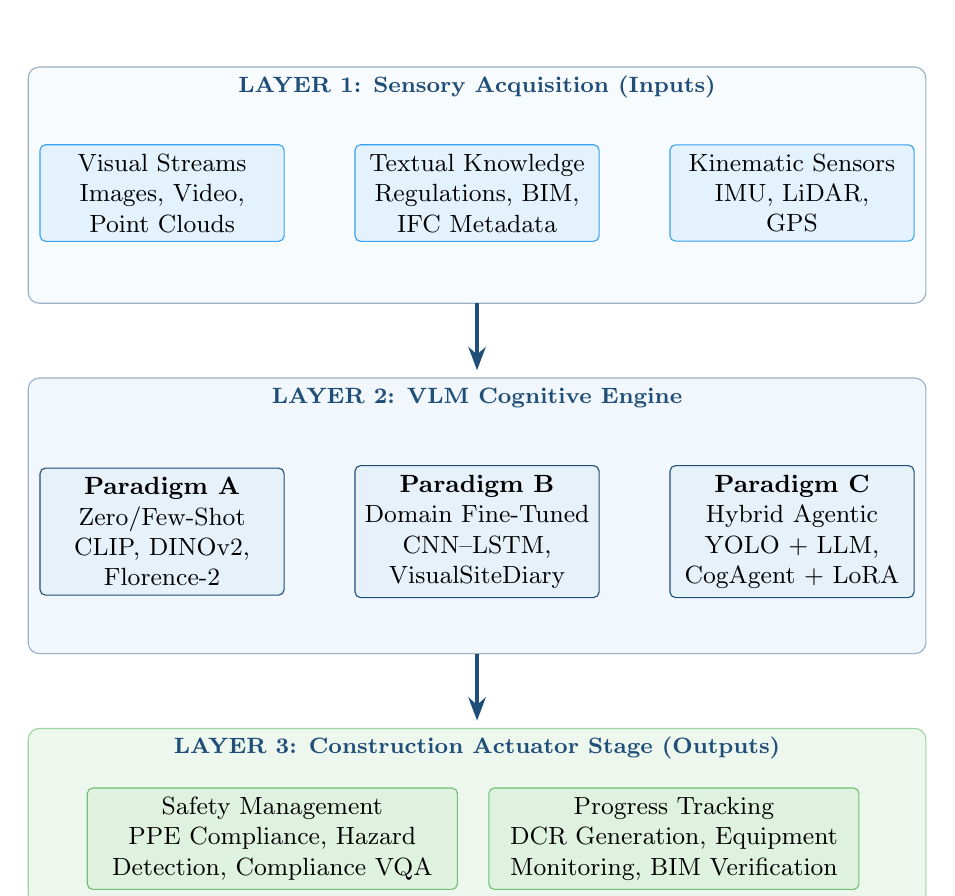
\begin{tikzpicture}[
  inp/.style={rectangle, draw=chartblue!90, fill=chartblue!12,
              rounded corners=2pt, minimum width=3.1cm, minimum height=1.1cm,
              align=center, font=\small},
  eng/.style={rectangle, draw=headingblue, fill=lightblue!65,
              rounded corners=2pt, minimum width=3.1cm, minimum height=1.6cm,
              align=center, font=\small},
  onode/.style={rectangle, draw=chartgreen!80, fill=chartgreen!18,
              rounded corners=2pt, minimum width=4.7cm, minimum height=1.2cm,
              align=center, font=\small},
  arr/.style={-Stealth, very thick, color=headingblue},
  hdr/.style={font=\footnotesize\bfseries\color{headingblue}},
]
%% --- Layer 1 background ---
\fill[lightblue!18, rounded corners=4pt] (-0.3, 1.0) rectangle (11.1, -2.0);
\draw[headingblue!45, rounded corners=4pt] (-0.3, 1.0) rectangle (11.1, -2.0);
\node[hdr] at (5.4, 0.75) {LAYER 1: Sensory Acquisition (Inputs)};

\node[inp] (i1) at (1.4, -0.6) {Visual Streams\\Images, Video,\\Point Clouds};
\node[inp] (i2) at (5.4, -0.6) {Textual Knowledge\\Regulations, BIM,\\IFC Metadata};
\node[inp] (i3) at (9.4, -0.6) {Kinematic Sensors\\IMU, LiDAR,\\GPS};

%% --- Arrow L1 → L2 ---
\draw[arr] (5.4,-2.0) -- (5.4,-2.85);

%% --- Layer 2 background ---
\fill[lightblue!38, rounded corners=4pt] (-0.3, -2.95) rectangle (11.1, -6.45);
\draw[headingblue!45, rounded corners=4pt] (-0.3, -2.95) rectangle (11.1, -6.45);
\node[hdr] at (5.4, -3.2) {LAYER 2: VLM Cognitive Engine};

\node[eng] (pa) at (1.4, -4.9) {\textbf{Paradigm A}\\Zero/Few-Shot\\CLIP, DINOv2,\\Florence-2};
\node[eng] (pb) at (5.4, -4.9) {\textbf{Paradigm B}\\Domain Fine-Tuned\\CNN--LSTM,\\VisualSiteDiary};
\node[eng] (pc) at (9.4, -4.9) {\textbf{Paradigm C}\\Hybrid Agentic\\YOLO + LLM,\\CogAgent + LoRA};

%% --- Arrow L2 → L3 ---
\draw[arr] (5.4,-6.45) -- (5.4,-7.3);

%% --- Layer 3 background ---
\fill[chartgreen!10, rounded corners=4pt] (-0.3, -7.4) rectangle (11.1, -9.65);
\draw[chartgreen!55, rounded corners=4pt] (-0.3, -7.4) rectangle (11.1, -9.65);
\node[hdr] at (5.4, -7.65) {LAYER 3: Construction Actuator Stage (Outputs)};

\node[onode] (o1) at (2.8, -8.8) {Safety Management\\PPE Compliance, Hazard\\Detection, Compliance VQA};
\node[onode] (o2) at (7.9, -8.8) {Progress Tracking\\DCR Generation, Equipment\\Monitoring, BIM Verification};
\end{tikzpicture}
\end{figure}

\subsection{Paradigm A: Zero/Few-Shot Prompting (Retrieval-Oriented)}

The deployment of traditional computer vision on construction sites has historically been bottlenecked by the need for extensive annotated datasets. Because traditional supervised learning methods suffer from high annotation costs, severe computational demands, and limited datasets, scaling these systems to cover every potential hazard or piece of equipment has proven prohibitively labor-intensive \cite{zhang2025}. To circumvent this strict reliance on massive data collection, studies from 2022 onward increasingly deployed foundational VLMs, such as Contrastive Language-Image Pre-training (CLIP), DINOv2, and Florence-2. Rather than relying on rigid numerical labels defined during a lengthy training phase, these multimodal methods acquire generalized visual representations guided by natural language supervision, enabling impressive zero-shot detection capabilities without requiring task-specific retraining \cite{zhang2025}.

Zero-shot retrieval operates by embedding both visual and textual inputs into a shared semantic space, allowing natural language to guide visual perception without any domain-specific labeled data. Contrastive pre-training enables a model to recognize an unseen class from its text description alone \cite{gil2024}; cosine similarity between visual features and text prompts replaces the traditional classification head \cite{liang2024}. This architecture is task-agnostic by design: by altering the textual query, the same model can recognize temporary construction site objects \cite{liang2024}, track heavy earthmoving equipment states \cite{jeoung2025}, or verify PPE compliance through semantic similarity scoring \cite{gil2024}. Open-vocabulary models such as Florence-2 extend this further, detecting any object described in a natural language prompt without being constrained to predefined classes \cite{jeoung2025}.

Zero-shot retrieval solves data scarcity but introduces a new limitation: its output is always a label or a similarity score, never a sentence. Because these models output discrete object locations and isolated class tags, they cannot generate the human-readable narratives that site managers need to understand what is actually happening on site \cite{bui2026}. This descriptive ceiling (retrieval without narration) is the specific gap that Paradigm~B addresses through generative fine-tuning.

\subsection{Paradigm B: Domain Fine-Tuned Generative Models}

To overcome the descriptive gap left by zero-shot retrieval models, subsequent studies addressed this descriptive gap by adopting image captioning architectures. Unlike traditional object detection that merely outputs discrete labels, image captioning combines computer vision and NLP to translate visual information into comprehensive natural language descriptions \cite{liu2020}. Generative fine-tuning operates through an encoder-decoder framework: a visual encoder extracts image features and a language decoder generates natural language sequences \cite{xiao2022}. Training on domain-specific construction datasets allows these architectures to acquire construction vocabulary and translate complex site scenes into human-readable narratives \cite{liu2020}.

Generative language output unlocked two capabilities that zero-shot retrieval could not provide: proactive hazard documentation and automated daily reporting. For safety management, pairing object detection with captioning enabled systems to generate descriptive text that proactively identifies hazards by matching visual scene descriptions against text-based safety rules \cite{wangxiao2024}. For progress tracking, detector-free Vision-Language Transformer architectures such as VisualSiteDiary automatically caption site photologs, extracting actionable insights about the ``where,'' ``how,'' and ``what'' of daily construction activity to support Daily Construction Report generation \cite{jung2024}.

Generative fine-tuning produces richer output than retrieval, but it remains a one-way system: the model describes what it sees, and the user receives that description without recourse. Workers and inspectors need to ask follow-up questions and probe specific details---none of which a static captioning pipeline supports \cite{chen2024}. This interactivity gap (narration without dialogue) is what Paradigm~C resolves through agentic hybrid stacks.

\subsection{Paradigm C: Hybrid Geometric-Semantic Systems (Agentic \& Hybrid Stacks)}

To overcome the interactive bottleneck of static image captioning, recent studies deployed agentic Large Multimodal Models (MLLMs). While previous paradigms successfully described scenes, they struggled to correlate visual observations directly with complex regulatory codes due to inherent limitations in geometric reasoning \cite{hussain2026}. To bridge this gap, Paradigm C introduces hybrid frameworks that combine precise geometric reasoning (such as bounding box coordinates or Building Information Modeling data) with LLM-powered interpretation to achieve true, regulation-aware scene understanding \cite{hussain2026}.

Hybrid systems achieve regulation-aware reasoning by fusing geometric detection outputs with large language model interpretation. Object detectors---typically YOLO variants---extract precise bounding-box coordinates of workers and equipment, which are then formatted as structured text prompts and passed to an MLLM for semantic interpretation \cite{hussain2026}. This pipeline supports two-way interactive dialogue: the model generates safety captions and responds to follow-up queries in natural language \cite{hussain2026}. To prevent hallucination and enforce regulatory accuracy, researchers have embedded construction safety ontologies directly into the prompting framework, constraining the MLLM to industry-standard language and enabling multi-step compliance checks such as verifying three-point contact or secure anchorage attachment \cite{chan2025}.

Paradigm~C has extended VLM capability across both the temporal and spatial dimensions of site management. Temporally, processing multiple consecutive video frames enables spatial inference, task classification, and event-level analysis---allowing a model to determine not just what an excavator is, but what task it is performing and how long it has been idle \cite{jeoung2025}. Spatially, integrating a VLM with a quadruped robot and BIM data creates a fully autonomous inspection loop: as the robot navigates the site, the VLM compares captured images against IFC metadata to determine whether architectural elements are present and correctly installed \cite{tuomisto2026}.

However, while Paradigm C represents the cutting edge of spatiotemporal construction scene understanding, it is not without critical vulnerabilities. The literature explicitly notes that despite significant progress in compliance checking, these advanced models are still challenged by dynamic scenarios and complex behavioral detection \cite{hussain2026}. Furthermore, their reliance on complex prompt engineering and their sensitivity to environmental noise introduces new risks of latency and unreliability in safety-critical settings.

\subsection{Layer 3: Construction Site Applications}

The architectural paradigms mapped in Sections~4.2--4.4 define what a VLM can produce; the application domain determines what it should produce. Layer~3 of the Three-Layered Framework---the actuator stage---translates each paradigm's cognitive outputs into construction management deliverables. The architectural paradigm constrains what outputs are achievable. Zero-shot retrieval (Paradigm~A) supports object identification and compliance checks without labeled training data. Generative fine-tuning (Paradigm~B) enables descriptive site documentation and daily reporting. Hybrid agentic stacks (Paradigm~C) unlock interactive inspection, regulatory reasoning, and temporal event monitoring. The following two subsections examine how these outputs operate across the two principal site management domains covered by this review.

\subsubsection{Construction Safety and Risk Management}

PPE compliance was the first construction safety task to benefit from zero-shot retrieval, because it maps naturally onto text-visual matching: does the worker's appearance match a natural language description of required equipment? Paradigm~A systems achieved this without labeled training data by extracting skeletal key points, cropping body-part images, and comparing generated captions against OSHA regulation prompts via cosine similarity \cite{gil2024}. However, PPE presence alone does not establish safety: workers may be fully equipped yet still engage in high-risk behaviors arising from complex spatiotemporal interactions. Comprehensive hazard management therefore requires moving beyond object-level checks toward contextual behavioral analysis.

To comprehensively capture these risky interactions, subsequent studies deployed Paradigm~B domain fine-tuned generative models to analyze unsafe behaviors. By pairing object detection with image captioning, safety systems gained the ability to generate rich textual descriptions of active scenes. These descriptions were matched against text-based safety rules to proactively identify hazards \cite{wangxiao2024}. Yet, despite successfully generating descriptive safety narratives, these systems remained static and lacked context-specific, interactive feedback essential for workers to fully comprehend their surrounding environments \cite{chen2024}.

Where Paradigm~B systems produced static safety narratives, Paradigm~C hybrid systems enabled interactive, regulation-aware monitoring by combining geometric detection with conversational LLMs. Augmented Reality integration extended this further: the VCSQ system embeds real-time captioning and VQA into a head-mounted display, allowing workers to query surrounding hazards on demand rather than waiting for a centralized inspection cycle \cite{chen2024}. To prevent hallucination and enforce regulatory compliance, ontology-driven prompting frameworks inject construction safety knowledge directly into the model's context, enabling multi-step compliance verification such as work-at-height regulation checking \cite{chan2025}. Mobile deployment extended the same architecture to site inspectors, where object detection feeds geometric coordinates into an LLM to generate hazard captions and support interactive safety dialogue \cite{hussain2026}.

Despite this progression, current VLMs still struggle with nuanced behavioral interpretation. Distinguishing whether a crew is effectively collaborating or merely communicating in proximity remains beyond reliable automated assessment \cite{bui2026}. Safety and productivity, however, share the same visual scene. The architectural investments made for hazard detection---temporal reasoning, spatial grounding, language-guided querying---directly transfer to progress tracking, which the following subsection examines.

\subsubsection{Progress Tracking and Automated Reporting}

Automated progress tracking begins with a simpler problem than safety: locating resources on site. Zero-shot retrieval addresses this without annotation overhead by comparing visual features against open-source text labels. An ImageNet-based similarity cache combined with contrastive pre-training recognizes temporary construction objects with no task-specific retraining \cite{liang2024}. Training-free multimodal frameworks similarly fuse object detectors with foundation models to extract localized bounding boxes for specific tools and materials \cite{zhang2025}. However, knowing where a tool is does not explain what work is happening. This gap drove adoption of generative architectures for richer site understanding.

Automating the daily administrative burden of site logging required generative architectures capable of producing narrative-level descriptions rather than bounding boxes. Detector-free Vision-Language Transformers such as VisualSiteDiary fine-tune on diverse site photologs, extracting actionable insights about the ``where,'' ``how,'' and ``what'' of daily work to support automated Daily Construction Report generation \cite{jung2024}. The key advance of Paradigm~B for progress tracking is precisely this shift from detection to narration: the output---narratives, not bounding boxes---arrives ready for site managers to use without additional interpretation.

Daily snapshots, however, cannot capture construction progress as it actually unfolds over time. Long-horizon equipment monitoring requires processing sequential frames over minutes or hours, not isolated images. Zero-shot temporal frameworks address this by evaluating multiple-choice questions about spatial position, task state, and event timing. Without task-specific training, these models determine what an excavator is doing and when a dump truck sits idle \cite{jeoung2025}.

Temporal querying answers the what-and-when question for individual equipment units. Spatial completeness requires a different integration: confirming whether every architectural element across a floor plate is physically present and correctly installed demands site-level coverage that temporal analysis alone cannot provide. Cutting-edge automated inspection frameworks address this by coupling conversational MLLMs with quadruped robots and BIM data \cite{tuomisto2026}. As the robot navigates partially built environments, an integrated foundational vision-language model acts as a virtual inspector, analyzing visual data against metadata extracted directly from the Industry Foundation Classes (IFC) model. Comparing captured images against IFC metadata, the VLM delivers programmatic binary assessments on whether each element is present, correctly positioned, and properly installed. This process bridges the digital twin and physical reality in real time \cite{tuomisto2026}.

% ============================================================
\section{Discussion and Limitations}
% ============================================================
\label{sec:discussion}

\subsection{Discussion}

Across 56 studies spanning 2010--2026, this review identifies a coherent multi-stage progression: from unimodal object detection and text-based compliance checking, through generative captioning and automated reporting, toward agentic hybrid systems capable of interactive, regulation-aware scene understanding. The four research questions yield the following findings.

\textbf{RQ1 (Architectures):} The literature reveals three distinct architectural paradigms (Paradigm A--C), each representing a progressive resolution of the semantic gap between visual data and construction management meaning. Paradigm A (CLIP, DINOv2, Florence-2) resolved the data-scarcity problem through zero-shot and few-shot retrieval but remained limited to discrete object tags. Paradigm B (CNN--LSTM, transformer-based captioning) introduced generative language output, enabling human-readable scene descriptions and automated daily logs but lacked interactivity. Paradigm C (YOLO + MLLM + ontology hybrid stacks, BIM-integrated robot VLMs) represents the most architecturally complete tier, enabling multi-turn dialogue, compliance verification, and temporal event analysis. The field has thus moved from a single-modal localization paradigm toward a genuinely multimodal decision-support architecture. However, Paradigm C studies are still predominantly prototypes rather than deployed systems.

\textbf{RQ2 (Multimodal Data Fusion):} Across the 20 core VLM studies, visual-text fusion is the dominant modality combination (17 of 20 studies), confirming that the core innovation of this generation of construction AI is the structured alignment of visual evidence with natural language: through shared embedding spaces (Paradigm A), encoder--decoder text generation (Paradigm B), or detect-then-prompt pipelines (Paradigm C). Temporal and geometric modalities are notably underrepresented: only 13 of 56 studies use video inputs, and only 5 incorporate geometric sensor data (LiDAR, IMU, or BIM). This gap directly shapes the field's current weakness in long-horizon activity monitoring, where sequential frame understanding is necessary but rarely achieved.

\textbf{RQ3 (Deployment Barriers):} Five recurring methodological bottlenecks emerge across the corpus. First, domain shift is the most universally reported limitation. This refers to the mismatch between models trained on general internet imagery and those deployed on construction sites, where object categories, lighting conditions, occlusion patterns, and domain terminology differ substantially. Second, data scarcity restricts the training and evaluation of domain-specific models; 85\% of core VLM studies relied on private custom datasets, preventing direct benchmarking. Third, prompt sensitivity in agentic Paradigm C systems introduces reliability risks in safety-critical contexts: minor prompt rewording can substantially alter model outputs. Fourth, real-site validation is systematically absent; the majority of studies evaluate on curated lab images or controlled video clips rather than unstructured field footage. Fifth, temporal reasoning remains the most technically underdeveloped capability. Understanding what is happening continuously over time, rather than at individual frames or short clips, is addressed by only one study in the corpus: Jeoung et al.\ (2025), which directly targets long-horizon equipment task monitoring.

\textbf{RQ4 (Evaluation):} Evaluation practice across the corpus is fragmented. No unified benchmark dataset or shared task specification exists for VLM-based construction monitoring. Detection metrics, NLG metrics, classification accuracy, and user studies are applied inconsistently across studies, making comparative assessment of progress impossible. The trend toward user-study evaluation in Paradigm C studies reflects a genuine shift toward human-centered assessment, but it introduces subjectivity and limits reproducibility. The absence of a shared benchmark reflects the field's immaturity. No agreed-upon task definitions yet exist for what ``good'' safety monitoring or progress tracking performance means in operational terms.

Taken together, these four findings point to a single overarching interpretation. The construction VLM field has demonstrated compelling proof-of-concept capability across safety inspection, progress reporting, PPE compliance, equipment monitoring, and interactive querying, but has not yet transitioned from laboratory demonstration to reliable field deployment. The practitioners' central question remains unanswered: can this system be trusted in an active construction environment? Human-in-the-loop deployment, with VLMs serving as assistive tools rather than autonomous decision-makers, is the most defensible near-term application model.

\subsection{Limitations}

This review has several constraints that readers should bear in mind when interpreting the findings. First, as a scoping review, it maps the extent and nature of the literature without evaluating study quality, effect sizes, or the relative merit of specific architectures. Claims about which paradigm ``works best'' are outside this review's scope. Second, the search was conducted on 4 March 2026; given the rapid publication pace in this domain, studies accepted after that cutoff are not represented, and some findings may already be superseded. Third, the literature is geographically concentrated: 69\% of papers originate from mainland China ($n=20$), South Korea ($n=6$), or the United States ($n=13$), which may introduce cultural and operational biases into the construction scenarios studied (e.g., building typology, safety regulation systems). Fourth, the English-language restriction may have excluded relevant work published in Chinese, Korean, or other languages. Fifth, the backward snowballing strategy, while necessary to capture foundational baseline work, may have introduced a citation bias toward frequently referenced earlier studies, inadvertently underrepresenting newer independent work. Sixth, as a scoping review, this study treats all included studies as methodologically equivalent regardless of sample size, study design, or validation rigor; future systematic reviews should incorporate formal quality appraisal to differentiate evidential weight. Seventh, data charting was conducted by the primary researcher without independent verification, which may have introduced subjective classification bias, particularly in paradigm assignments for architecturally borderline cases.

% ============================================================
\section{Conclusion}
% ============================================================

This scoping review mapped 56 peer-reviewed studies to characterize the current state of Vision-Language Model (VLM) and multimodal AI applications for construction site safety monitoring and progress tracking. The review reveals a field in active transition: unimodal computer vision, which dominated prior-generation monitoring systems, is being systematically replaced by multimodal architectures that fuse visual perception with natural language reasoning. This transition has unfolded in three identifiable stages. First, retrieval-oriented zero-shot models use language to guide visual search. Second, generative domain-fine-tuned captioning pipelines produce human-readable site reports. Third, agentic hybrid stacks integrate object detectors, large multimodal models, and domain ontologies into interactive, regulation-aware inspection systems.

The review makes three primary contributions to the field. First, it presents, to the authors' knowledge, the first PRISMA-ScR scoping review to explicitly map VLM architectural paradigms as applied to active construction safety and progress monitoring, organized around a Three-Layered Spatiotemporal VLM Framework (sensory inputs, cognitive engine, and actionable outputs) that offers a reusable classification tool for future research. Second, it explicitly answers four foundational research questions covering architectural prevalence, multimodal fusion strategies, deployment barriers, and evaluation practices. This synthesis covers a heterogeneous corpus that prior construction AI reviews have not mapped at the paradigm level. Third, it identifies the field's most critical gaps: the absence of shared construction-specific benchmarks, the underdevelopment of long-horizon temporal reasoning, the near-universal reliance on private datasets, and the systematic absence of real-site field validation.

For researchers, these gaps define a near-term research agenda. Construction-specific VLM benchmark datasets represent the highest-leverage investment the field could make. These datasets should cover safety compliance, equipment task classification, and temporal activity chains on real sites. For practitioners, the current evidence base supports the use of VLMs as assistive inspection tools, with human verification required for any safety-critical decision. Full-autonomy deployment remains premature given the current state of prompt sensitivity, domain shift, and real-site reliability data. These insights highlight both the substantial progress that VLMs represent relative to unimodal predecessors and the clear distance that remains before this technology delivers reliable, field-validated performance across the diversity of actual construction environments.

\begin{thebibliography}{99}

\bibitem{alaloul2022} Alaloul, W.~S., Alzubi, K.~M., Malkawi, A.~B., Al Salaheen, M., and Musarat, M.~A. (2022). ``Productivity monitoring in building construction projects: A systematic review.'' \textit{Engineering, Construction and Architectural Management}, 29(7), 2760--2785. \href{https://doi.org/10.1108/ECAM-12-2020-1074}{DOI: 10.1108/ECAM-12-2020-1074}

\bibitem{asadzadeh2020} Asadzadeh, A., Arashpour, M., Li, H., Ngo, T., Bab-Hadiashar, A., and Rashidi, A. (2020). ``Sensor-based safety management.'' \textit{Automation in Construction}, 113, 103128. \href{https://doi.org/10.1016/j.autcon.2020.103128}{DOI: 10.1016/j.autcon.2020.103128}

\bibitem{bang2020} Bang, S., and Kim, H. (2020). ``Context-based information generation for managing UAV-acquired data using image captioning.'' \textit{Automation in Construction}, 112, 103116. \href{https://doi.org/10.1016/j.autcon.2020.103116}{DOI: 10.1016/j.autcon.2020.103116}

\bibitem{bohn2010} Bohn, J.~S., and Teizer, J. (2010). ``Benefits and barriers of construction project monitoring using high-resolution automated cameras.'' \textit{Journal of Construction Engineering and Management}, 136(6), 632--640. \href{https://doi.org/10.1061/(ASCE)CO.1943-7862.0000167}{DOI: 10.1061/(ASCE)CO.1943-7862.0000167}

\bibitem{bui2026} Bui, H.~T., Chodosh, N.~E., and Tavakoli, A. (2026). ``Can vision-language models understand construction workers? An exploratory study.'' arXiv preprint arXiv:2601.10835. \href{https://arxiv.org/abs/2601.10835}{arXiv: 2601.10835}

\bibitem{chan2025} Chan, C.-F., Wong, P.~K.-Y., Guo, X., Cheng, J.~C.~P., Chan, J.~P.-C., Leung, P.-H., and Tao, X. (2025). ``Context-aware vision-language model agent enriched with domain-specific ontology for construction site safety monitoring.'' \textit{Automation in Construction}, 177, 106305. \href{https://doi.org/10.1016/j.autcon.2025.106305}{DOI: 10.1016/j.autcon.2025.106305}

\bibitem{chenc2023} Chen, C., Xiao, B., Zhang, Y., and Zhu, Z. (2023). ``Automatic vision-based calculation of excavator earthmoving productivity using zero-shot learning activity recognition.'' \textit{Automation in Construction}, 146, 104702. \href{https://doi.org/10.1016/j.autcon.2022.104702}{DOI: 10.1016/j.autcon.2022.104702}

\bibitem{chen2024} Chen, H., Hou, L., Wu, S., Zhang, G., Zou, Y., Moon, S., and Bhuiyan, M. (2024). ``Augmented reality, deep learning and vision-language query system for construction worker safety.'' \textit{Automation in Construction}, 157, 105158. \href{https://doi.org/10.1016/j.autcon.2023.105158}{DOI: 10.1016/j.autcon.2023.105158}

\bibitem{davila2021} Davila Delgado, J.~M., and Oyedele, L. (2021). ``Deep learning with small datasets: Using autoencoders to address limited datasets in construction management.'' \textit{Applied Soft Computing}, 112, 107836. \href{https://doi.org/10.1016/j.asoc.2021.107836}{DOI: 10.1016/j.asoc.2021.107836}

\bibitem{gil2024} Gil, M., and Lee, S. (2024). ``Zero-shot monitoring of construction workers' personal protective equipment based on image captioning.'' \textit{Automation in Construction}, 164, 105470. \href{https://doi.org/10.1016/j.autcon.2024.105470}{DOI: 10.1016/j.autcon.2024.105470}

\bibitem{hussain2026} Hussain, R., Lee, D., Abbas, M.~S., Zaidi, S.~F.~A., Pedro, A., and Park, C. (2026). ``Vision-language model-based intelligent assistant for onsite construction safety inspection.'' \textit{Automation in Construction}, 182, 106728. \href{https://doi.org/10.1016/j.autcon.2025.106728}{DOI: 10.1016/j.autcon.2025.106728}

\bibitem{jang2025} Jang, J., Cha, M., Park, M., and Kim, H. (2025). ``Transformer-based deep learning model and video dataset for installation action recognition in offsite projects.'' \textit{Automation in Construction}, 172, 106042. \href{https://doi.org/10.1016/j.autcon.2025.106042}{DOI: 10.1016/j.autcon.2025.106042}

\bibitem{jeoung2025} Jeoung, H., Jung, M., and Kim, C. (2025). ``Zero-shot framework for construction equipment task monitoring.'' \textit{Computer-Aided Civil and Infrastructure Engineering}. \href{https://doi.org/10.1111/mice.13506}{DOI: 10.1111/mice.13506}

\bibitem{jiang2023} Jiang, Z., and Messner, J.~I. (2023). ``Computer vision applications in construction and asset management phases: A literature review.'' \textit{Journal of Information Technology in Construction (ITcon)}, 28(9), 176--199. \href{https://doi.org/10.36680/j.itcon.2023.009}{DOI: 10.36680/j.itcon.2023.009}

\bibitem{jung2024} Jung, Y., Cho, I., Hsu, S.-H., and Golparvar-Fard, M. (2024). ``VisualSiteDiary: A detector-free vision-language transformer model for captioning photologs for daily construction reporting and image retrievals.'' \textit{Automation in Construction}, 165, 105483. \href{https://doi.org/10.1016/j.autcon.2024.105483}{DOI: 10.1016/j.autcon.2024.105483}

\bibitem{li2025} Li, H., Deng, H., and Deng, Y. (2025). ``Towards worker-centric construction scene understanding: Status quo and future directions.'' \textit{Automation in Construction}, 171, 106005. \href{https://doi.org/10.1016/j.autcon.2025.106005}{DOI: 10.1016/j.autcon.2025.106005}

\bibitem{liang2024} Liang, Y., et al. (2024). ``Recognizing temporary construction site objects using CLIP-based few-shot learning and multi-modal prototypes.'' \textit{Automation in Construction}, 165, 105542. \href{https://doi.org/10.1016/j.autcon.2024.105542}{DOI: 10.1016/j.autcon.2024.105542}

\bibitem{liu2020} Liu, H., Wang, G., Huang, T., He, P., Skitmore, M., and Luo, X. (2020). ``Manifesting construction activity scenes via image captioning.'' \textit{Automation in Construction}, 119, 103334. \href{https://doi.org/10.1016/j.autcon.2020.103334}{DOI: 10.1016/j.autcon.2020.103334}

\bibitem{nath2020} Nath, N.~D., Behzadan, A.~H., and Paal, S.~G. (2020). ``Deep learning for site safety: Real-time detection of personal protective equipment.'' \textit{Automation in Construction}, 112, 103085. \href{https://doi.org/10.1016/j.autcon.2020.103085}{DOI: 10.1016/j.autcon.2020.103085}

\bibitem{paneru2021} Paneru, S., and Jeelani, I. (2021). ``Computer vision applications in construction: Current state, opportunities \& challenges.'' \textit{Automation in Construction}, 132, 103940. \href{https://doi.org/10.1016/j.autcon.2021.103940}{DOI: 10.1016/j.autcon.2021.103940}

\bibitem{parasuraman2000} Parasuraman, R., Sheridan, T.~B., and Wickens, C.~D. (2000). ``A model for types and levels of human interaction with automation.'' \textit{IEEE Transactions on Systems, Man, and Cybernetics -- Part A}, 30(3), 286--297. \href{https://doi.org/10.1109/3468.844354}{DOI: 10.1109/3468.844354}

\bibitem{rabbi2024} Rabbi, A.~B.~K., and Jeelani, I. (2024). ``AI integration in construction safety: Current state, challenges, and future opportunities in text, vision, and audio based applications.'' \textit{Automation in Construction}, 164, 105443. \href{https://doi.org/10.1016/j.autcon.2024.105443}{DOI: 10.1016/j.autcon.2024.105443}

\bibitem{samsami2024} Samsami, R. (2024). ``A systematic review of automated construction inspection and progress monitoring (ACIPM): Applications, challenges, and future directions.'' \textit{CivilEng}, 5(1), 265--287. \href{https://doi.org/10.3390/civileng5010014}{DOI: 10.3390/civileng5010014}

\bibitem{sherafat2020} Sherafat, B., Ahn, C.~R., Akhavian, R., Behzadan, A.~H., Golparvar-Fard, M., Kim, H., Lee, Y.-C., Rashidi, A., and Rezazadeh Azar, E. (2020). ``Automated methods for activity recognition of construction workers and equipment: State-of-the-art review.'' \textit{Journal of Construction Engineering and Management}, 146(6), 03120002. \href{https://doi.org/10.1061/(ASCE)CO.1943-7862.0001843}{DOI: 10.1061/(ASCE)CO.1943-7862.0001843}

\bibitem{sun2024} Sun, Y., Gu, Z., and Yang, S.~B. (2024). ``Probing vision and language models for construction waste material recognition.'' \textit{Automation in Construction}, 166, 105629. \href{https://doi.org/10.1016/j.autcon.2024.105629}{DOI: 10.1016/j.autcon.2024.105629}

\bibitem{tohidifar2024} Tohidifar, A., Kim, D., and Lee, S. (2024). ``Make it till you fake it: Construction-centric computational framework for simultaneous image synthetization and multimodal labeling.'' \textit{Automation in Construction}, 167, 105696. \href{https://doi.org/10.1016/j.autcon.2024.105696}{DOI: 10.1016/j.autcon.2024.105696}

\bibitem{tricco2018} Tricco, A.~C., Lillie, E., Zarin, W., O'Brien, K.~K., et al. (2018). ``PRISMA extension for scoping reviews (PRISMA-ScR): Checklist and explanation.'' \textit{Annals of Internal Medicine}, 169(7), 467--473. \href{https://doi.org/10.7326/M18-0850}{DOI: 10.7326/M18-0850}

\bibitem{tuomisto2026} Tuomisto, J., Zheng, Y., Chauhan, I., Sepp\"anen, O., and Pajarinen, J. (2026). ``Automating on-site object inspection with a quadruped robot and BIM.'' \textit{Automation in Construction}, 181, 106571. \href{https://doi.org/10.1016/j.autcon.2025.106571}{DOI: 10.1016/j.autcon.2025.106571}

\bibitem{wang2023} Wang, X., and El-Gohary, N. (2023). ``Deep learning-based relation extraction and knowledge graph-based representation of construction safety requirements.'' \textit{Automation in Construction}, 147, 104696. \href{https://doi.org/10.1016/j.autcon.2022.104696}{DOI: 10.1016/j.autcon.2022.104696}

\bibitem{wang2024} Wang, X., and El-Gohary, N. (2024). ``Few-shot object detection and attribute recognition from construction site images for improved field compliance.'' \textit{Automation in Construction}, 167, 105539. \href{https://doi.org/10.1016/j.autcon.2024.105539}{DOI: 10.1016/j.autcon.2024.105539}

\bibitem{wangb2024} Wang, B., Chen, Z., Li, M., Wang, Q., Yin, C., and Cheng, J.~C.~P. (2024). ``Omni-Scan2BIM: A ready-to-use Scan2BIM approach based on vision foundation models for MEP scenes.'' \textit{Automation in Construction}, 162, 105384. \href{https://doi.org/10.1016/j.autcon.2024.105384}{DOI: 10.1016/j.autcon.2024.105384}

\bibitem{wangxiao2024} Wang, Y., Xiao, B., Bouferguene, A., and Al-Hussein, M. (2024). ``Proactive safety hazard identification using visual--text semantic similarity for construction safety management.'' \textit{Automation in Construction}, 166, 105602. \href{https://doi.org/10.1016/j.autcon.2024.105602}{DOI: 10.1016/j.autcon.2024.105602}

\bibitem{wu2021} Wu, H., Zhong, B., Li, H., Love, P., Pan, X., and Zhao, N. (2021). ``Combining computer vision with semantic reasoning for on-site safety management in construction.'' \textit{Journal of Building Engineering}, 42, 103036. \href{https://doi.org/10.1016/j.jobe.2021.103036}{DOI: 10.1016/j.jobe.2021.103036}

\bibitem{xiao2022} Xiao, B., Wang, Y., and Kang, S.-C. (2022). ``Deep learning image captioning in construction management: A feasibility study.'' \textit{Journal of Construction Engineering and Management}, 148(7), 04022049. \href{https://doi.org/10.1061/(ASCE)CO.1943-7862.0002297}{DOI: 10.1061/(ASCE)CO.1943-7862.0002297}

\bibitem{xiao2024} Xiao, B., Wang, Y., Zhang, Y., Chen, C., and Darko, A. (2024). ``Automated daily report generation from construction videos using ChatGPT and computer vision.'' \textit{Automation in Construction}, 168, 105874. \href{https://doi.org/10.1016/j.autcon.2024.105874}{DOI: 10.1016/j.autcon.2024.105874}

\bibitem{xin2024} Xin, C., Hartel, A., and Kasneci, E. (2024). ``DART: An automated end-to-end object detection pipeline with data diversification, open-vocabulary bounding box annotation, pseudo-label review, and model training.'' \textit{Expert Systems with Applications}, 258, 125124. \href{https://doi.org/10.1016/j.eswa.2024.125124}{DOI: 10.1016/j.eswa.2024.125124}

\bibitem{xiong2019} Xiong, R., Song, Y., Li, H., and Wang, Y. (2019). ``Onsite video mining for construction hazards identification with visual relationships.'' \textit{Advanced Engineering Informatics}, 42, 100966. \href{https://doi.org/10.1016/j.aei.2019.100966}{DOI: 10.1016/j.aei.2019.100966}

\bibitem{yang2023} Yang, M., Wu, C., Guo, Y., Jiang, R., Zhou, F., Zhang, J., and Yang, Z. (2023). ``Transformer-based deep learning model and video dataset for unsafe action identification in construction projects.'' \textit{Automation in Construction}, 146, 104703. \href{https://doi.org/10.1016/j.autcon.2022.104703}{DOI: 10.1016/j.autcon.2022.104703}

\bibitem{zhai2023} Zhai, P., Wang, J., and Zhang, L. (2023). ``Extracting worker unsafe behaviors from construction images using image captioning with deep learning--based attention mechanism.'' \textit{Journal of Construction Engineering and Management}, 149(2), 04022164. \href{https://doi.org/10.1061/JCEMD4.COENG-12096}{DOI: 10.1061/JCEMD4.COENG-12096}

\bibitem{zhang2015} Zhang, J., and El-Gohary, N.~M. (2015). ``Automated information transformation for automated regulatory compliance checking in construction.'' \textit{Journal of Computing in Civil Engineering}, 29(4), B4015001. \href{https://doi.org/10.1061/(ASCE)CP.1943-5487.0000427}{DOI: 10.1061/(ASCE)CP.1943-5487.0000427}

\bibitem{zhang2025} Zhang, Z., Yu, Y., Pan, Z., and Antwi-Afari, M.~F. (2025). ``Training-free few-shot construction tool and material detection using pre-trained vision-language model.'' \textit{Computer-Aided Civil and Infrastructure Engineering}, 40(30), 6004--6023. \href{https://doi.org/10.1111/mice.13326}{DOI: 10.1111/mice.13326}

\bibitem{zhong2019} Zhong, B., Wu, H., Ding, L., Love, P.~E.~D., Li, H., Luo, H., and Jiao, L. (2019). ``Mapping computer vision research in construction: Developments, knowledge gaps and implications for research.'' \textit{Automation in Construction}, 107, 102919. \href{https://doi.org/10.1016/j.autcon.2019.102919}{DOI: 10.1016/j.autcon.2019.102919}

\end{thebibliography}

\end{document}
